\documentclass[conference]{IEEEtran}
%\IEEEoverridecommandlockouts
% The preceding line is only needed to identify funding in the first footnote. If that is unneeded, please comment it out.
\usepackage{cite}
\usepackage{amsmath,amssymb,amsfonts}
\usepackage{algorithmic}
\usepackage{graphicx}
\usepackage{textcomp}
\usepackage{xcolor}
\usepackage{subcaption}
\def\BibTeX{{\rm B\kern-.05em{\sc i\kern-.025em b}\kern-.08em
    T\kern-.1667em\lower.7ex\hbox{E}\kern-.125emX}}
\begin{document}

\title{Kalman and Particle filter's robustness to non-linearity}

\author{
    \IEEEauthorblockN{Marius Oechslein}
    \IEEEauthorblockA{
        \textit{Faculty of Computer Science and Business Information Systems} \\
        \textit{University of Applied Sciences Würzburg-Schweinfurt}\\
        Würzburg, Germany \\
        marius.oechslein@study.thws.de
    }
        %\and
}
\maketitle

\begin{abstract}

The Kalman and Particle filters are widely used techniques for estimating positions based on noisy observations.
In this study, we examine the behavior of these filters in the context of a ball throw with a nonlinear trajectory.
While the Kalman filter is not expected to accurately model nonlinearity, the Particle filter is well-suited for such problems.

Firstly, we investigate how the Kalman filter behaves precisely at the point of nonlinearity, which occurs when the ball hits the wall.
Secondly, we test the robustness of the Particle filter as the nonlinearity of the system increases. 
	This is accomplished by altering the number of observations and their variance as more walls are introduced, thereby increasing the level of nonlinearity.

\end{abstract}

\begin{IEEEkeywords}
Particle Filter, Kalman Filter, Ball Throw, Non-linearity, Robustness
\end{IEEEkeywords}

\section{Introduction}
The trajectory of a ball captured by a 2D camera, which involves noisy observations, can be effectively modeled using the Kalman and Particle filters.
Both filters are applicable in this scenario due to the inherent uncertainty associated with the noisy observations.

The Kalman filter is well-suited for accurately modeling linear systems and offers the advantage of computationally efficient calculations \cite{b6}.
Conversely, the Particle filter is capable of modeling such a problem by iteratively estimating the ball's most probable position over time \cite{b3}.

In order to introduce non-linearity into this setup, we incorporate walls that alter the ball's direction upon impact.
However, the fundamental assumptions of the Kalman filter indicate that it may struggle to accurately model such non-linear systems.
Therefore, it is interesting to investigate how the Kalman filter exactly behaves in such situations. 

On the other hand, the Particle filter is widely used for scenarios involving non-linear systems \cite{b3}.
To assess the robustness of the Particle filter in non-linear systems, we conduct two experiments.
Firstly, we decrease the number of observations, and secondly, we increase the variance of the observations.
The key focus is to determine the impact of these variations on the Particle filter's robustness.


\section{Physics of a ball throw}


To accurately estimate the position of a thrown ball in the next time step, the physics of ball throwing must be incorporated into the state transition.
The x-position can be modeled as follows:
\begin{equation*}
    \begin{aligned}
    x_{t+1} = x_{t} + v_x * \Delta t,   \\
    x, v_x \in \mathbb{R}
    \end{aligned}
    \tag{1}
\end{equation*}
Here, ${v_x}$ represents the ball's constant velocity in the x-direction, and $x_t$ denotes the x-position of the ball at time step t.

On the other hand, determining the position and velocity in the y-direction is slightly more complex due to the influence of gravity. 
The equation is given by:
\begin{equation*}
    \begin{aligned}
    y_{t+1} = y_t + v_y \Delta t - 0.5 g \Delta t^2, \\
    y, v_y \in \mathbb{R}
    \end{aligned}
    \tag{2}
\end{equation*}
In this equation, g represents the gravitational constant $g = 9.81$.

When the ball hits a wall, the only change in the physical motion is that the velocity in the x-direction must be negated.
Therefore, at the time step corresponding to the position of the wall, the x-velocity should be updated as follows: $x^{vel} = -x^{vel}$.
The velocity in the y-direction remains unchanged, assuming that there is no fraction upon impact and that the wall is perfectly vertical.
The equation for the x-position also remains unaffected.


\section{Kalman and Particle filter}
In this section the Kalman and Particle filter are presented. 
% TODO: equations for the kalman and particles filters
For both the Kalman and Particle filter the hidden state is defined as follows:
\begin{equation*}
\textbf{q} = (x, y, v_x, v_y)   \tag{3}
\end{equation*}
Only the x and y-positions are incorporated in the observations, given by:
\begin{equation*}
    \begin{aligned}
    \textbf{o} = (x, y)
    \end{aligned}
\tag{4}
\end{equation*}

Both Kalman and Particle filters implement the following equation for the recursive density estimation:
\begin{equation*}
    p(\textbf{q}_t | \langle \textbf{o} \rangle _t) =
    p(\textbf{o}_t | \textbf{q}_t) \int p(\textbf{q}_t | \textbf{q}_{t-1}) p(\textbf{q}_{t-1} | \langle \textbf{q} \rangle _{t-1}) d \textbf{q}_{t-1}
\tag{5}
\end{equation*}

The Kalman filter achieves this through the utilization of the Kalman gain algorithm \cite{b2}.
A crucial characteristic of the Kalman filter is its assumption of linearity.
Consequently, the Kalman filter is incapable of modeling non-linear systems \cite{b2}.
On the contrary, the Particle filter is equipped to handle non-linearities and can be implemented using the Condensation algorithm \cite{b3}.


\subsection{Experimental setup}

The first experiment focuses on a ball throw scenario where the ball collides with a wall positioned 50 meters away.
This experiment aims to assess the ability of the Kalman and Particle filters to model this non-linearity.
The expected outcome is that the Kalman filter will struggle to capture the non-linearity, while the Particle filter is anticipated to handle it effectively.
Of particular interest the behavior of the Kalman filter at the time step when the ball hits the wall and shortly thereafter.

The second experiment aims to evaluate the robustness of the Particle filter as the level of non-linearity in the system increases.
To amplify the non-linearity, two additional walls are introduced.
The objective is to investigate the Particle filter's robustness as the non-linearity increases.
To test the robustness, two experiments with modified parameters are conducted: reducing the number of observations and increasing the variance of the noise in the observations.

The decision to solely modify the variance and number of observations was based on the primary focus of examining the Particle filter's ability to track the trajectory.
While other parameters such as noise distribution and assumed starting position could have been altered, it would have been unnecessary since the variance and number of observations already provide valuable insights into the Particle filter's robustness.
All noise was assumed to follow a normal distribution, and the starting positions were set to the actual starting positions of the ball.

% TODO:
%\begin{figure}[h]
%\centerline{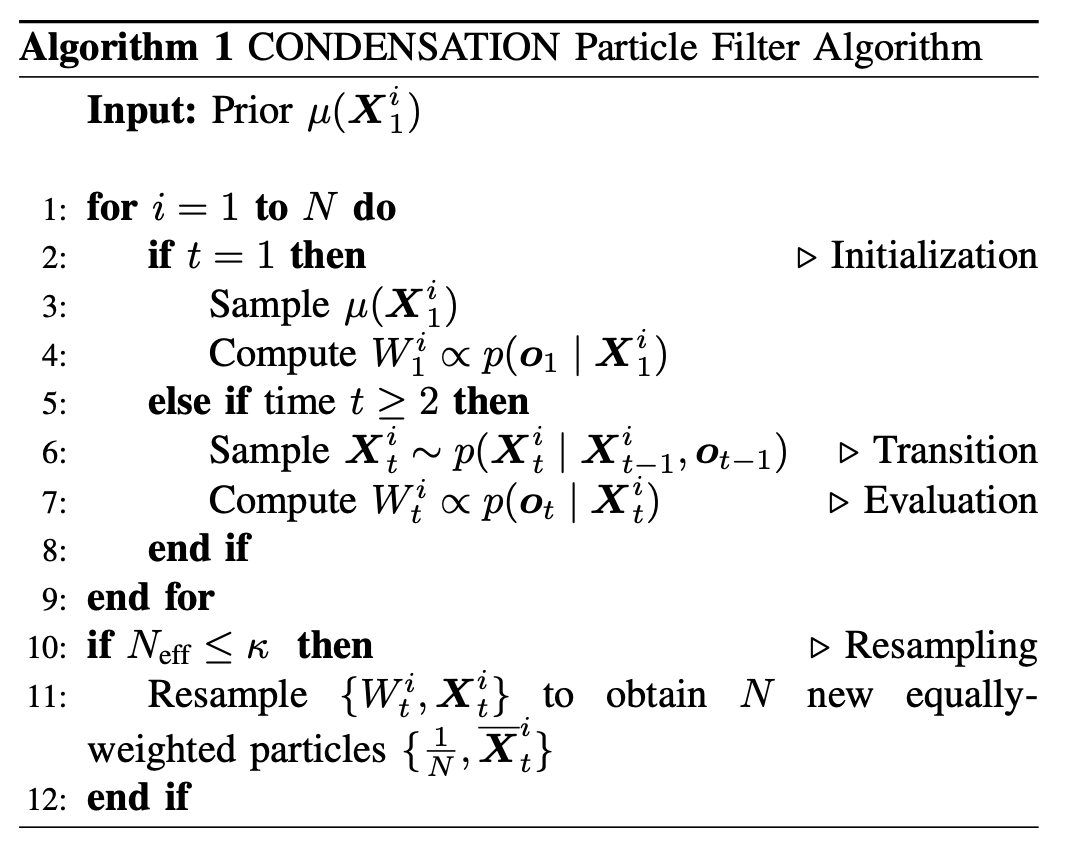
\includegraphics[width=70mm]{figs/condensation-algorithm.png}}
%\caption{Condensation Particle filter algorithm from \cite{b1}.}
%\label{fig:condensation-algorithm}
%\end{figure}


\section{Results}

% Kalman filter with time_sim=5, time_step=0.1, variance=1
% Particle filter 1 boundary normal: time=5, time_step=0.1, variance=1
% Particle filter 1 boundary high variance: time=5, time_step=0.1, variance=8 -> 50 observations
% Particle filter 1 boundary few observations: time=5, time_step=0.1, variance=1 -> 12 observations
% Kalman filter 3 boundaries: time_sim=5, time_step=0.1, variance=1
% Particle filter 3 boundaries normal: time=5, time_step=0.025, variance=0.5 -> 200 observations! and lower variance
% Particle filter 3 boundaries higher variance: time=5, time_step=0.025, variance=1 -> way worse for only a little bit more noise
% Particle filter 3 boundaries fewer observations: time=5, time_step=0.1, variance=0.5 -> 50 observations

\subsection{Kalman and Particle Filter modelling non-linearities}

First, the results of the Kalman filter's position estimation for the ball are presented.
\begin{figure}
	\centering
	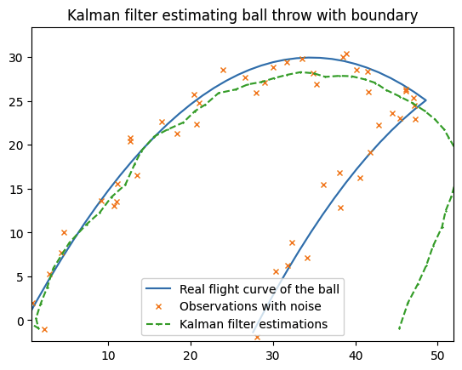
\includegraphics[width=70mm]{figs/kalman-filter.png}
	\caption{Kalman filter modelling non-linearities. From own calculations.}
	\label{fig:kalman-filter}
\end{figure}

In fig. \ref{fig:kalman-filter}, it is evident that the Kalman filter effectively models the trajectory of the ball until the point of impact with the wall.
However, following the collision, the Kalman filter's estimations continue along the same trajectory.
As the errors increase over each time step, the Kalman filter changes its direction slowly, but is never able to come close to the real positions again.

In contrast, the Particle filter demonstrates impressive performance in modeling the non-linearity, as illustrated in Figure \ref{fig:particle-filter-one-boundary}.
It accurately estimates the ball's positions both before and after the wall collision, effectively tracking its trajectory.

It is important to note that, in both experiments, the variance of the observation noise and the number of observations are kept the same to enable a comparison of the two filters.
\begin{table}[htbp]
    \caption{Estimation errors for one boundary. Boundary 50 m away.}
    \begin{center}
    \begin{tabular}{|c|c|c|}
    \cline{1-3}
    & Before hitting the wall & After hitting the wall \\
    \cline{1-3} 
    Kalman filter & \textit{1.2 m} & \textit{17.73 m} \\
    \cline{1-3} 
    Particle filter & \textit{1.87 m} & \textit{3.01 m} \\
    \hline
    \end{tabular}
    \label{tab:comparing-kalman-particle}
    \end{center}
\end{table}

As the ball hits the wall, the estimation errors increase for both the Kalman and Particle filters, as shown in Table \ref{tab:comparing-kalman-particle}.
However, the Particle filter maintains a consistent level of low error throughout, while the Kalman filter experiences a drastic increase in error after the ball hits the wall.
Although the Kalman filter demonstrates slightly higher accuracy of approximately 0.5 meters compared to the Particle filter before the wall impact, this difference is not significant, as it may be due to the uncertainties of the system.


\subsection{Robustness of the Particle filter with increasing non-linearity}

In this section, the focus is on examining the robustness of the Particle filter as the level of non-linearity increases by adding two more walls.

To establish a baseline performance, the Particle filter is initially tested with reasonable values for the variance and number of observations.
Subsequently, these parameters are adjusted to assess the filter's robustness.

\begin{figure}
	\centering
	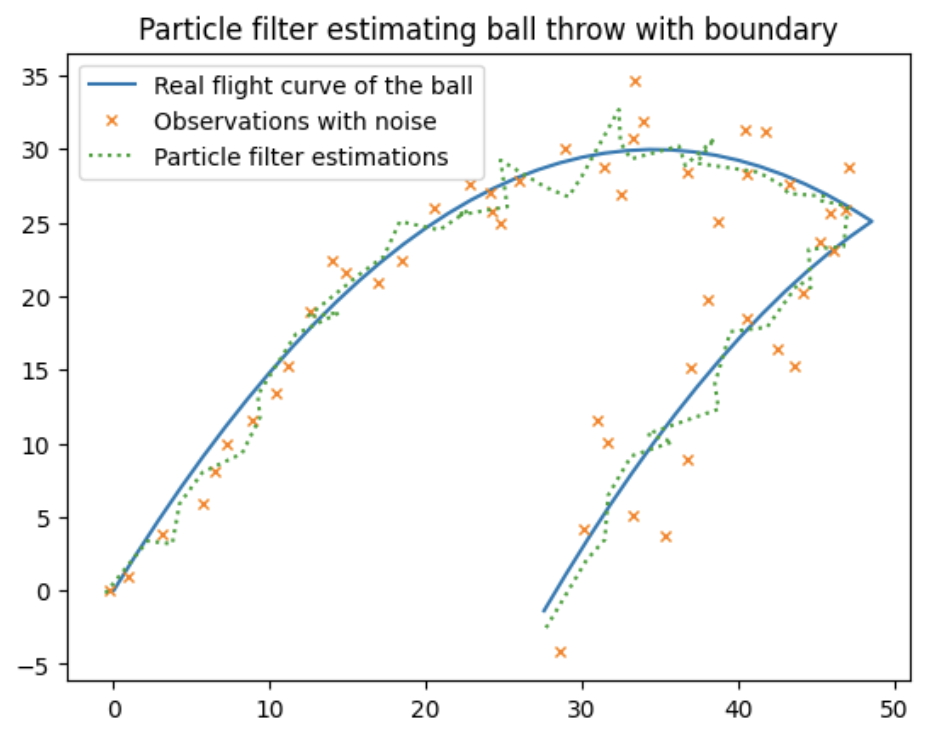
\includegraphics[width=70mm]{figs/particle-filter-one-boundary}
	\caption{Particle filter with one boundary. From own calculations.}
	\label{fig:particle-filter-one-boundary}
\end{figure}
\begin{figure}
	\centering
	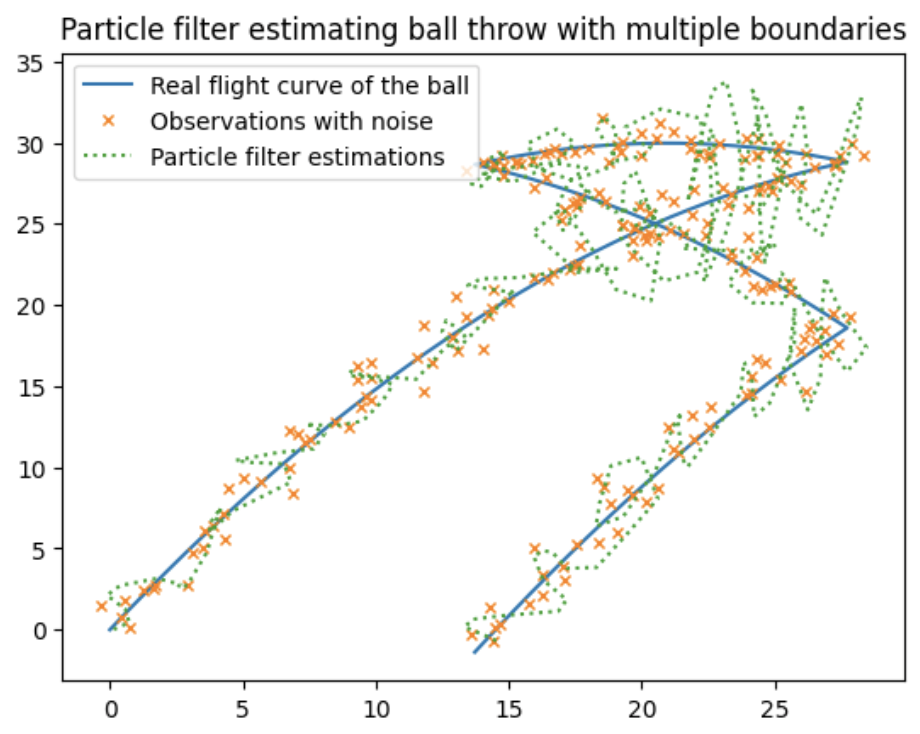
\includegraphics[width=70mm]{figs/particle-filter-multiple-boundaries}
	\caption{Particle filter with multiple boundaries. From own calculations.}
	\label{fig:particle-filter-multiple-boundaries}
\end{figure}

It should be noted that as two more walls are introduced, the variance needs to be reduced significantly and the number of observations increased substantially.
For the experiment with a single wall (fig. \ref{fig:particle-filter-one-boundary}), the noise variance is set to 1 and the number of observations is set to 50.
However, for the scenario with three walls (fig. \ref{fig:particle-filter-multiple-boundaries}), the variance had to be lowered to 0.025, while the number of observations had to be increased to 200 to achieve a reasonably accurate modeling of the ball's trajectory.
This indicates that the Particle filter becomes less robust in estimating the ball throw as the number of non-linearities increases.

\begin{figure}
	\centering
	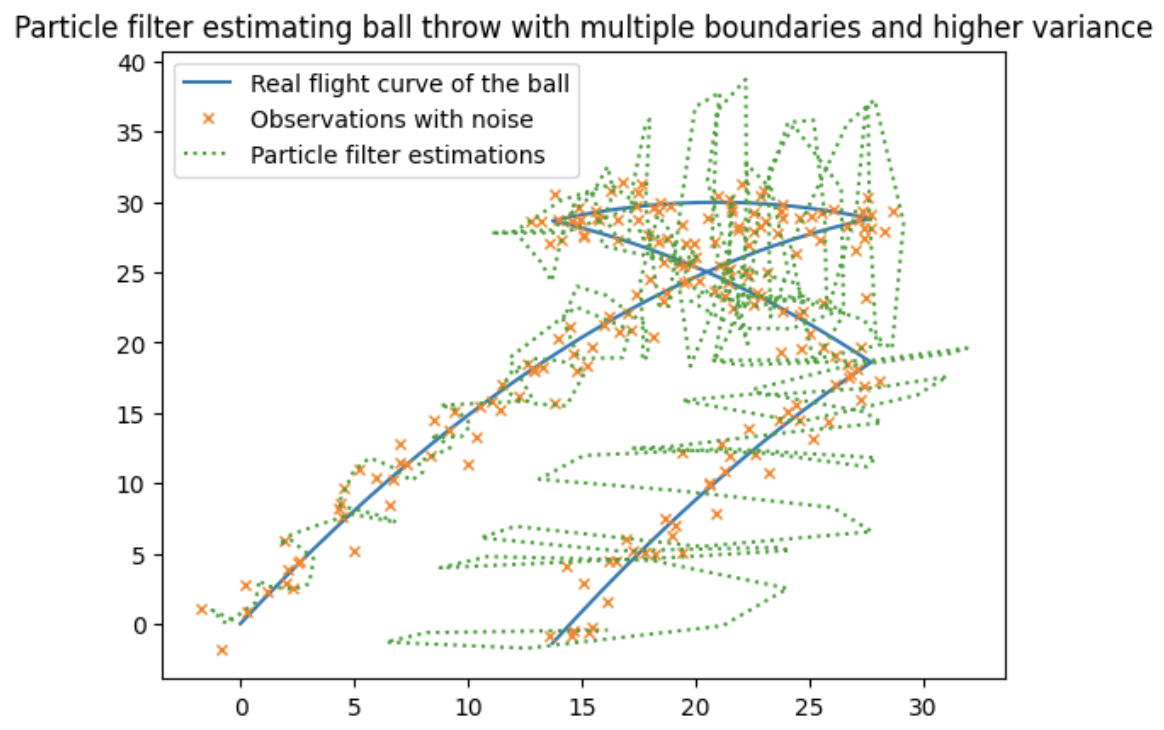
\includegraphics[width=70mm]{figs/particle-filter-multiple-boundaries-higher-variance}
	\caption{Particle filter with multiple boundaries and higher variance. From own calculations.}
	\label{fig:particle-filter-multiple-boundaries-higher-variance}
\end{figure}

Initially, the variance of the observation noise is increased from 0.025 to 1.
It is important to note that this is the same variance used in the experiment with a single boundary (fig. \ref{fig:particle-filter-one-boundary}).
The estimation results presented in fig. \ref{fig:particle-filter-multiple-boundaries-higher-variance} show a noticeable degradation compared to the experiment with a single wall, despite using the same variance for the noise.
This indicates a decrease in the robustness of the Particle filter as the level of non-linearity increases.

\begin{figure}
	\centering
	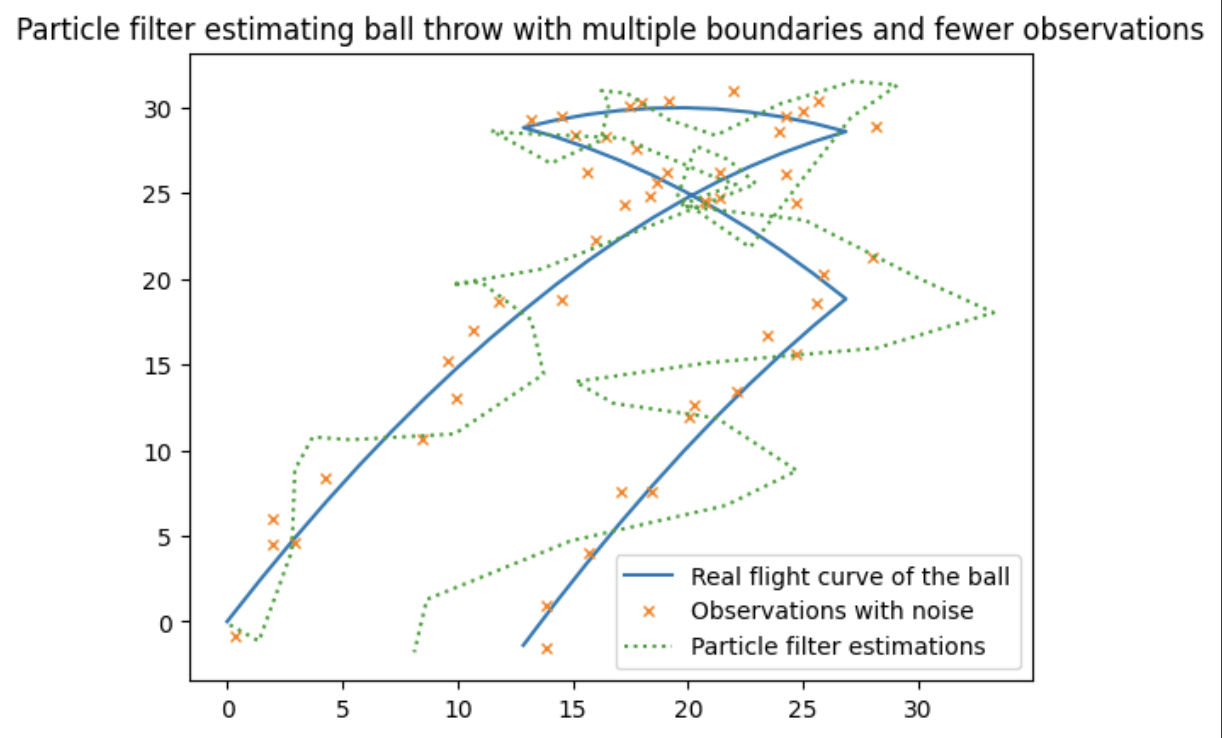
\includegraphics[width=70mm]{figs/particle-filter-multiple-boundaries-fewer-observations}
	\caption{Particle filter with multiple boundaries and fewer observations. From own calculations.}
	\label{fig:particle-filter-multiple-boundaries-fewer-observations}
\end{figure}

Next, the number of observations is decreased from 200 to 50.
Here again, it is worth mentioning that this corresponds to the same number of observations used in the experiment with a single boundary (fig. \ref{fig:particle-filter-one-boundary}).
The results shown in fig. \ref{fig:particle-filter-multiple-boundaries-fewer-observations} when reducing the number of observations reveal a similar trend as increasing the variance: the robustness of the model decreases as the level of non-linearity increases.

In conclusion, all the conducted experiments clearly demonstrate that the robustness of the Particle filter decreases as the non-linearity of the system increases.


\section{Discussion}\label{sec:discussion}

\subsection{Kalman and Particle Filter modelling non-linearities}

Due to the fundamental assumption of linearity in Kalman filters, they are incapable of effectively modeling non-linearities.
This limitation was also evident in the experiments conducted in this study.
To address the challenges posed by non-linear systems, various alternative non-linear filters have been proposed in literature, including particle filters, unscented Kalman filters, extended Kalman filters, batch filters, and exact recursive filters \cite{b5}.

While this paper specifically focused on investigating the Particle filter, the performance of other non-linear filters was not assessed.
It would be of interest for future research to explore whether these alternative non-linear filters would be able to model the non-linearity better.

\subsection{Robustness of the Particle filter with increasing non-linearity}
The Particle filter demonstrated superior modeling of non-linearity compared to the Kalman filter.
However, its robustness decreased as the level of non-linearity increased.
To maintain accurate modeling in the face of increased non-linearity, the Particle filter required more observations and reduced variance in the noise of the observations.

The findings of this study could be attributed to well-known challenges associated with Particle filters, which could impact their estimation performance.
These challenges include the Degeneracy Problem, Sample Impoverishment, Particle Filter Divergence, and the selection of the Importance Density \cite{b4}.
In this section, I will discuss how each of these challenges relates to the observed result of the Particle filter's reduced robustness with increasing non-linearity.


\subsection{Degeneracy Problem}
The Degeneracy Problem occurs when, after a few iterations, the weight becomes concentrated on a single particle while the weights of all other particles approach zero \cite{b4}.
To mitigate this issue, a resampling step is typically employed, wherein new particles are generated based on the weights of particles from the previous iteration.
In the implementation used in this paper, which utilizes the Condensation Algorithm \cite{b3}, this problem is already addressed.
Therefore, the Degeneracy Problem cannot be attributed as the cause of the observed results in high non-linearity cases.


\subsection{Sample Improverishment}
The resampling step, which aims to address the Degeneracy Problem, can itself become problematic.
During resampling, particles with high weights are duplicated, which can be problematic if the state transition fails to sufficiently diversify the new particle positions \cite{b4}.
This can lead to a situation where all particles collapse into a single position over time.

The Condensation algorithm used in this implementation does not specifically address this problem, which suggests that it may have influenced the results of the experiments in this paper.
In fig. \ref{fig:particle-filter-multiple-boundaries-higher-variance}, where the number of observations was increased to 200, the plot indicates a significant deterioration in the performance of the Particle filter over time.
This deterioration could be attributed to the Sample Improverishment problem, which occurs when all particles converge to a single point, resulting in poorer estimation over time \cite{b4}.

It is important to note that this problem does not necessarily break the Particle filter.
For instance, in fig. \ref{fig:particle-filter-multiple-boundaries}, where the number of observations is also increased to 200, the estimations are reasonably close to the actual positions.
However, this highlights that the Particle filter is not sufficiently robust for high non-linearity scenarios, as the estimations deteriorate significantly when the variance is increased or the number of observations is decreased.


\subsection{Particle Filter Divergence}
The third challenge is Particle Filter Divergence, which refers to the situation where the filter's estimations deviate significantly from the actual positions.
This problem can arise due to inadequate tuning of the filter, incorrect model assumptions, or issues with the measurements \cite{b4}.

In the context of this study, although the Particle filter encounters difficulties in modeling highly nonlinear systems, the estimations generally still approximate the real positions, albeit with significant errors.
However, the Particle Filter Divergence problem is unlikely to occur in this application.
This is because the ball throw dynamics are explicitly incorporated into the state transition, and the observations are artificially generated, thus preventing the occurrence of this problem.


\subsection{Selecting the Importance Density}

The selection of an appropriate Importance Density is crucial for the performance of the Particle filter, as it needs to align with the characteristics of the system being modeled \cite{b4}.
In this study, the use of a Gaussian distribution for generating observations is known, and a matching Gaussian distribution was employed for the Particle filter.
Therefore, the selection of the Importance Density is not considered a problem, as it is appropriately chosen to align with the underlying Gaussian distribution of the observations.


\section{Conclusion}

This paper conducted experiments to address two main research questions.

The first question aimed to investigate the behavior of the Kalman filter in a non-linear system.
The results demonstrated that the Kalman filter followed its estimated trajectory, even when the observed trajectory changed direction.
However, as the estimation errors accumulated, the Kalman filter slowly changed its estimation direction but it never returned to the correct position.

The second question focused on examining the impact of increasing non-linearity on the robustness of the Particle filter.
The findings indicated that the Particle filter's performance deteriorated as the non-linearity of the system increased.
This is an interesting conclusion which may be counter-intuitive.

Both the Kalman and Particle filters have their own limitations and various methods have been developed to address the challenges associated with each filter.
Further investigations could explore alternative methods, such as the Extended Kalman filter, which aims to address the non-linearity problem of the Kalman filter.
Additionally, exploring other techniques that aim to enhance the robustness of the Particle filter may shed light on potential improvements for this specific use case.

\begin{thebibliography}{00} % TODO: 
	\bibitem{b1} Fetzer, T., Bullmann, M., Ebner, M., Kastner, S., Deinzer, F., \& Grzegorzek, M. Interacting Multiple Model Particle Filter for Indoor Positioning Applications.
	\bibitem{b2} Thrun, S. (2002). Probabilistic robotics. Communications of the ACM, 45(3), 52-57. % TODO: Correct?
	\bibitem{b3} Isard, M., \& Blake, A. (1998). CONDENSATION--conditional density propagation for visual tracking. International journal of computer vision, 29(1), 5.
	\bibitem{b4} Elfring, J., Torta, E., \& van de Molengraft, R. (2021). Particle filters: A hands-on tutorial. Sensors, 21(2), 438.
	\bibitem{b5} Daum, F. (2005). Nonlinear filters: beyond the Kalman filter. IEEE Aerospace and Electronic Systems Magazine, 20(8), 57-69.
	\bibitem{b6} Welch, G., \& Bishop, G. (1995). An introduction to the Kalman filter.

\end{thebibliography}

\end{document}
